\section{Ablations}
\label{sec:ablations}
\subsection{Anchor ratio}
\label{sec:ablation-kappa}
\Cref{fig:kappa} sweeps $\kap$ from 0.1 to 10 on sparse-view CT. PSNR is flat for $\kap \in [0.5, 2]$ and falls off on both sides: too small a ratio starves the likelihood and the reconstruction drifts towards an unconditional sample, too large a ratio recovers the unanchored behaviour. We therefore use $\kap = 1$ everywhere and did not tune it per dataset.

\begin{figure}[t]
  \centering
  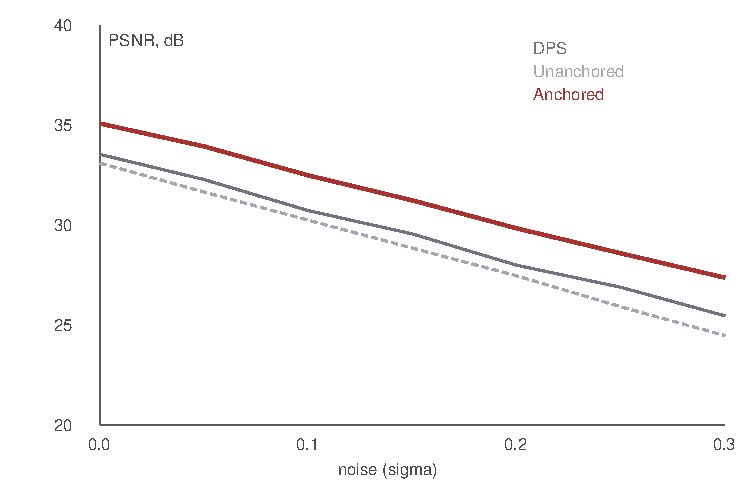
\includegraphics[width=\linewidth]{figures/kappa-sweep.pdf}
  \caption{PSNR against the anchor ratio $\kap$ on sparse-view CT at $\sigma = 0.1$. The plateau between 0.5 and 2 motivates the single value used in every experiment.}
  \label{fig:kappa}
\end{figure}

\subsection{Which norm}
\label{sec:ablation-norm}
Replacing the $\ell_2$ norm in \cref{eq:anchor} with $\ell_\infty$ changes PSNR by less than 0.1 dB; a per-pixel clip performs worse by 0.6 dB because it changes the direction of $g_t$. \Cref{tab:norm} has the numbers.
\begin{table}[t]
  \centering
  \caption{Choice of norm in the anchoring rule, sparse-view CT at $\sigma = 0.1$.}
  \label{tab:norm}
  \begin{tabular}{lc}
    \toprule
    Norm & PSNR (dB) \\
    \midrule
    $\ell_2$ (ours) & 33.8 \\
    $\ell_\infty$ & 33.7 \\
    Per-pixel clip & 33.2 \\
    \bottomrule
  \end{tabular}
\end{table}


\subsection{Sampler}
\label{sec:ablation-sampler}
\Cref{tab:sampler} compares DDIM with 100 steps, predictor--corrector with 1000 steps and the EDM stochastic sampler with 50 steps, each with and without anchoring. The margin from anchoring is between 1.4 and 2.1 dB in every case, so the rule does not depend on the sampler.
\begin{table}[t]
  \centering
  \caption{Anchoring across samplers, sparse-view CT at $\sigma = 0.1$.}
  \label{tab:sampler}
  \begin{tabular}{lcc}
    \toprule
    Sampler & Unanchored & Anchored \\
    \midrule
    DDIM, 100 steps & 31.0 & 32.9 \\
    Predictor--corrector, 1000 steps & 31.7 & 33.8 \\
    EDM stochastic, 50 steps & 31.4 & 32.8 \\
    \bottomrule
  \end{tabular}
\end{table}


\subsection{Schedule for the anchor ratio}
\label{sec:ablation-schedule}
A ratio that decays linearly from 2 to 0.5 over the reverse process matches the constant ratio to within 0.05 dB. We report the constant ratio because it has no schedule to tune.
